\section{The plug-in}
Here a step by step explanation will guide the user through the proper usage of the prediction plug-in.

\subsection{Loading the plug-in}
\begin{enumerate}
	\item the user will have to select the plus icon from the sidebar, from which a drop-down menu containing four options will appear; from this menu the "dashboard" option has to be selected;


\begin{figure}[H]
\centering
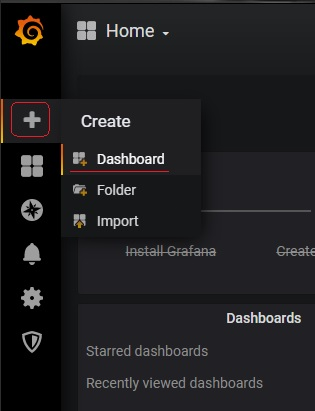
\includegraphics[scale=0.90]{img/plug-in/plus_dash.png}
\caption{Training operation with graphic point}
\end{figure}


	\item the user will now have to select the "Chose Visualization" button;


\begin{figure}[H]
\centering
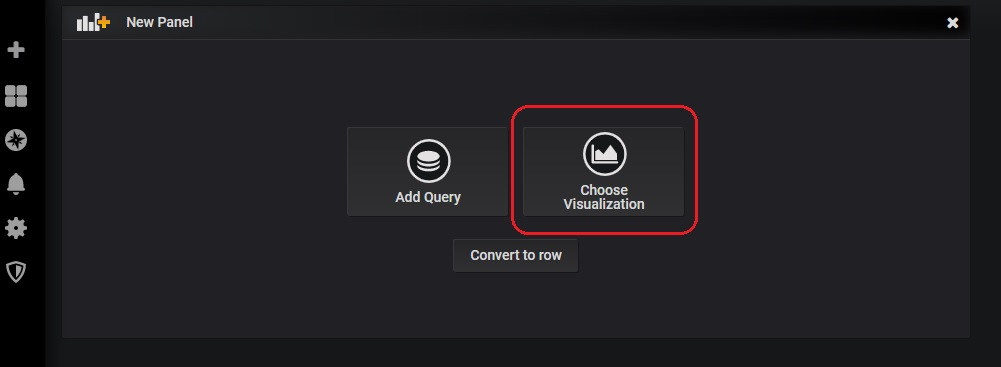
\includegraphics[scale=0.65]{img/plug-in/visual.png}
\caption{Chose Visualization button}
\end{figure}


	\item finally, by pressing on the "Predire in Grafana" button, the user can use the plug-in.
	
\begin{figure}[H]
\centering
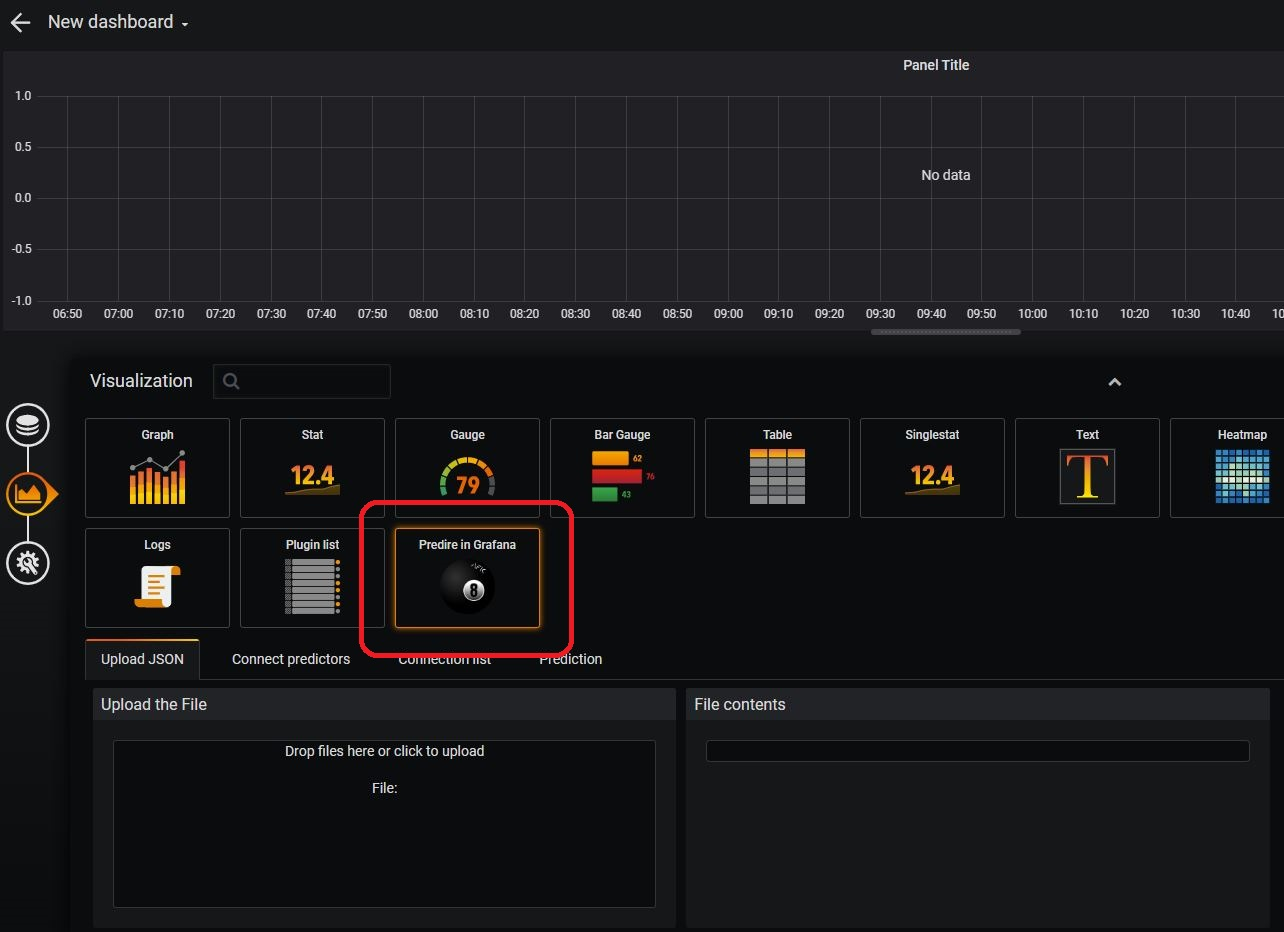
\includegraphics[scale=0.55]{img/plug-in/plugin_1.JPG}
\caption{"Predire in Grafana" Panel}
\end{figure}

\end{enumerate}

	
\subsection{Loading a JSON file}
The user can select the “Upload the file” button contained in the “Upload JSON” section.
This will open a window from which the JSON file can be selected.
Alternatively, the user can drag and drop the JSON file in the "Upload the file" section.
The content of the JSON file will be displayed in a panel called "File contents" to the right of the previously mentioned section.

\begin{figure}[H]
\centering
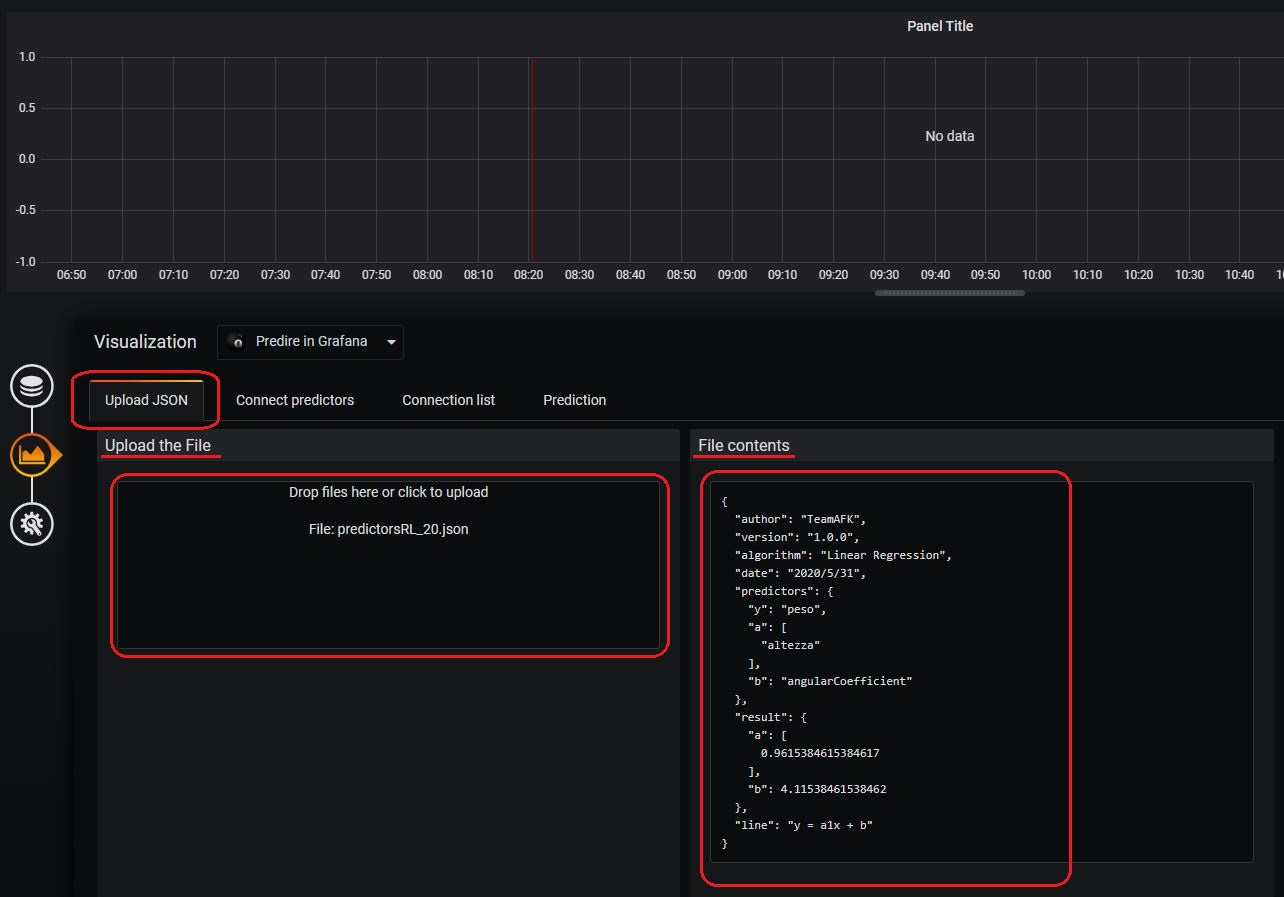
\includegraphics[scale=0.60]{img/plug-in/plugin_2.JPG}
\caption{Loading window and displayed loaded JSON}
\end{figure}


\subsection{Connecting predictors}
The portion of the software dedicated to the connection of the nodes can be accessed by selecting the "Connect predictors" tab:
\begin{enumerate}
	\item the user can choose from the “Insert connection” section which queries are to be associated with which nodes.
	Once all the nodes are connected, the user can select the "Add connection" button and confirm the operation;
	
\begin{figure}[H]
\centering
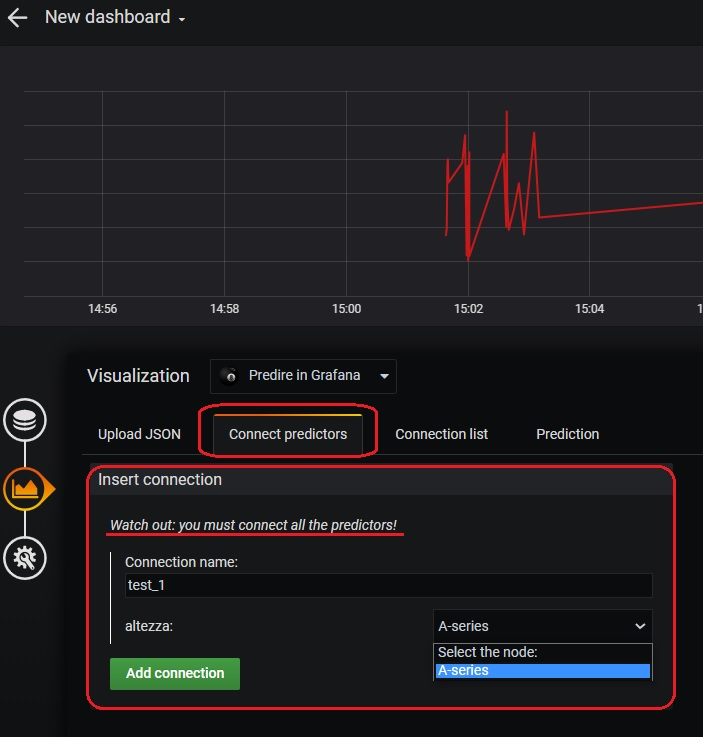
\includegraphics[scale=0.75]{img/plug-in/plugin_3.JPG}
\caption{Connection coupling (a)}
\end{figure}



\begin{enumerate}
\item should the user have not filled all the required fields, an error message will be displayed on selection of the "Add connection" button;

	
\begin{figure}[H]
\centering
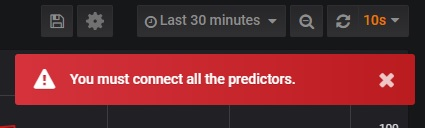
\includegraphics[scale=0.60]{img/plug-in/plugin_4.JPG}
\caption{Connection coupling error message}
\end{figure}

\item once all the required fields are correctly chosen, a confirm message will be displayed. 

\begin{figure}[H]
\centering
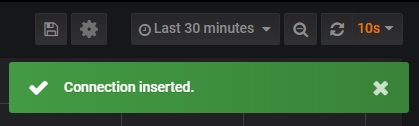
\includegraphics[scale=0.60]{img/plug-in/plugin_5.JPG}
\caption{Connection coupling confirm message}
\end{figure}

\end{enumerate} 


\end{enumerate}



\subsection{Modifying the connections}
In this section the user can view all the predictor-data stream connections that have been made. This section can be accessed by selecting the "Connection list" tab.
The user can also modify the connection, by pressing on the "Edit" button, or delete it, by selecting the "Disconnect" button.

\begin{figure}[H]
\centering
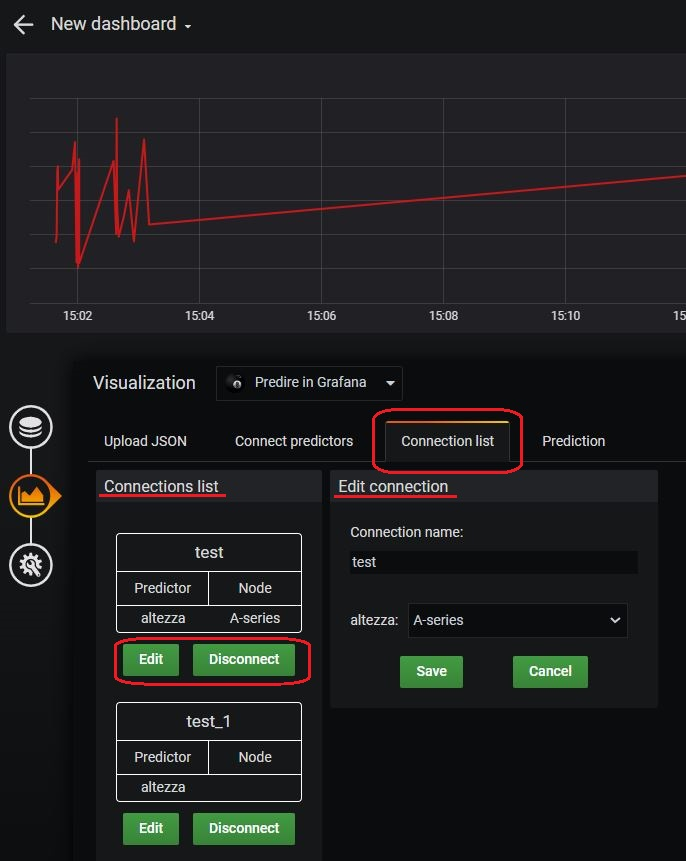
\includegraphics[scale=0.75]{img/plug-in/plugin_6.JPG}
\caption{Node linking}
\end{figure}


\subsection{Prediction operations}
In this last section the user will be able to launch the prediction algorithms of the plug-in. This section is accessed by selecting the "Prediction" tab. Here the user will be able to select, in the top right corner, a temporal policy by choosing starting and ending dates and choosing how often to sample the data. The user  also has access to two buttons, one called "Start monitoring", which starts the prediction operations, and a second one named "Enable saving", which saves the data collected up to the point it is pressed.\\

\begin{figure}[H]
\centering
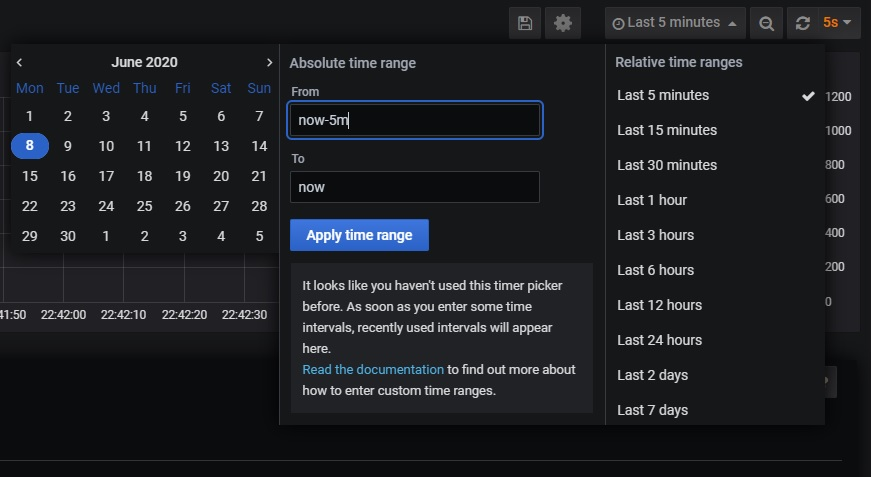
\includegraphics[scale=0.70]{img/plug-in/time_selector.png}
\caption{Time picker}
\end{figure}

When the prediction has been started, the "Start monitoring" button becomes "Stop monitoring", which, if pressed, will stop the monitoring.

\begin{figure}[H]
\centering
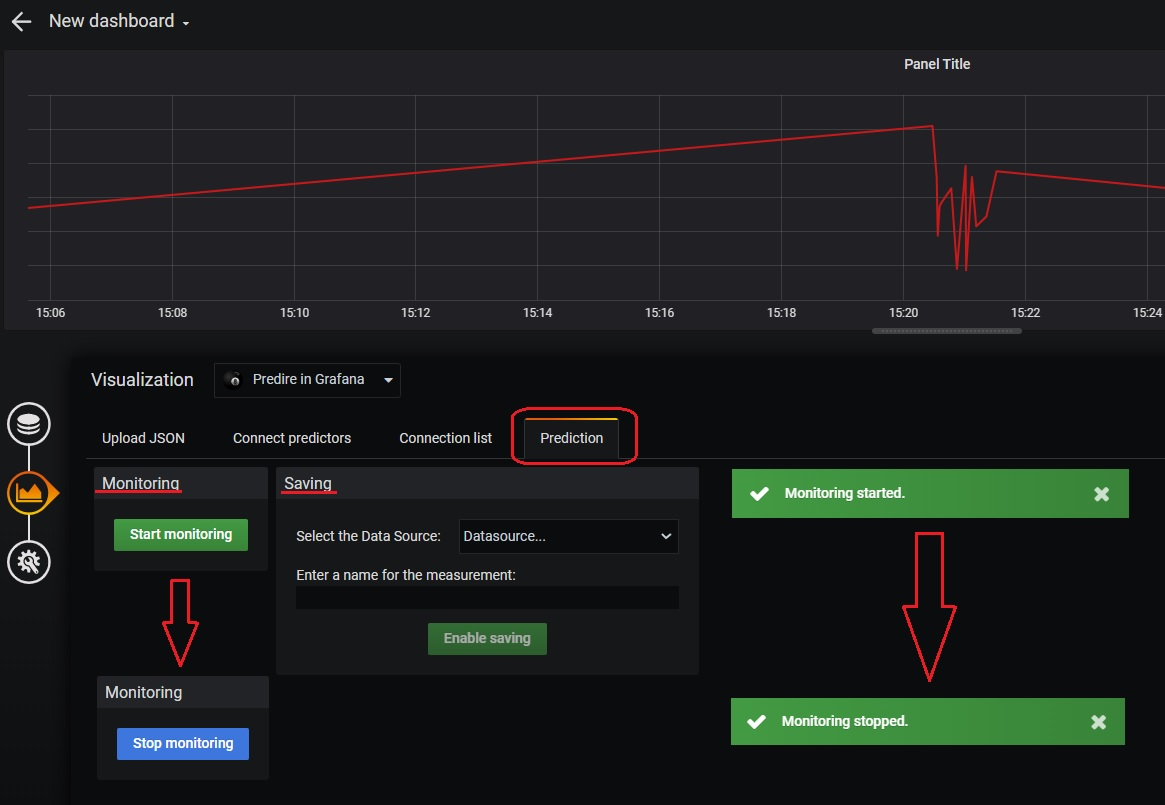
\includegraphics[scale=0.65]{img/plug-in/plugin_7.JPG}
\caption{Begin\textbackslash end data monitoring and Prediction save}

\end{figure} 
 

